\subsection{Systematic Parameter Selection}\label{sec:systematic-parameters}
This subsection provides a theoretically-grounded approach for parameter selection based on the analysis in Section~\ref{sec:theoretical-analysis}. Unlike heuristic approaches, our methodology establishes principled relationships between system properties and algorithm parameters, ensuring optimal performance across diverse applications.

\textbf{Parameter Optimization Framework:} Given system characteristics \( \{m, T_s, \sigma_\omega, L_c\} \) representing dimension, sampling time, noise level, and correlation length respectively, we determine optimal parameters through the following systematic approach:
\begin{figure}[H]
	\centering
	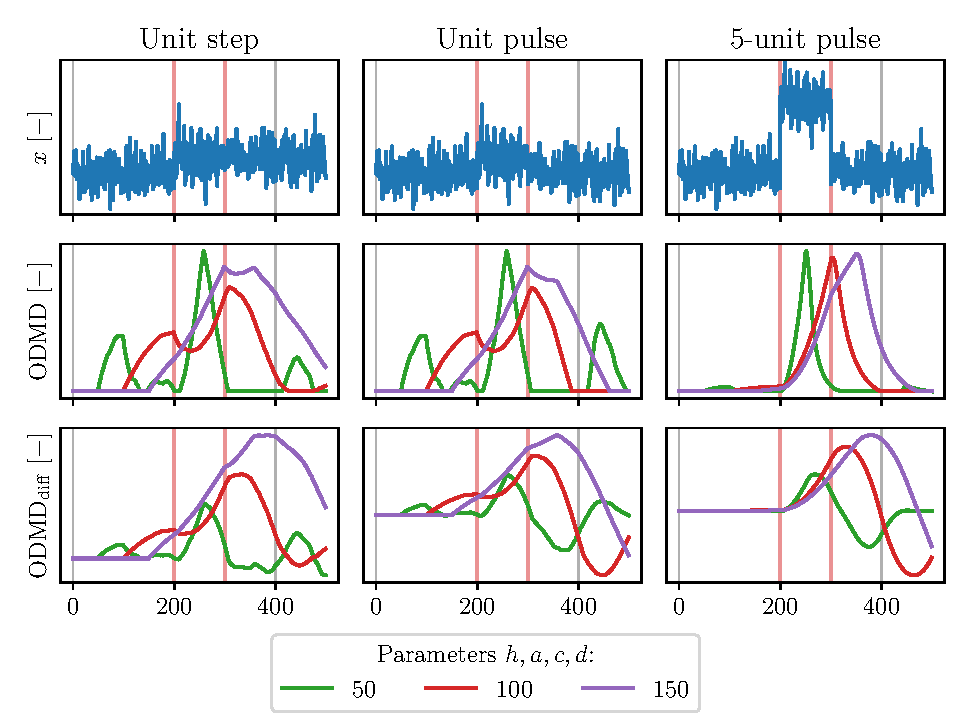
\includegraphics[width=\linewidth]{figures/parameters-influence-allatonce.pdf}
	\caption{Increasing value of all the hyperparameters at once increases robustness to noise and delays peak of CPD statistics.}\label{fig:hyperparameters-all}
\end{figure}

\begin{figure}[H]
	\centering
	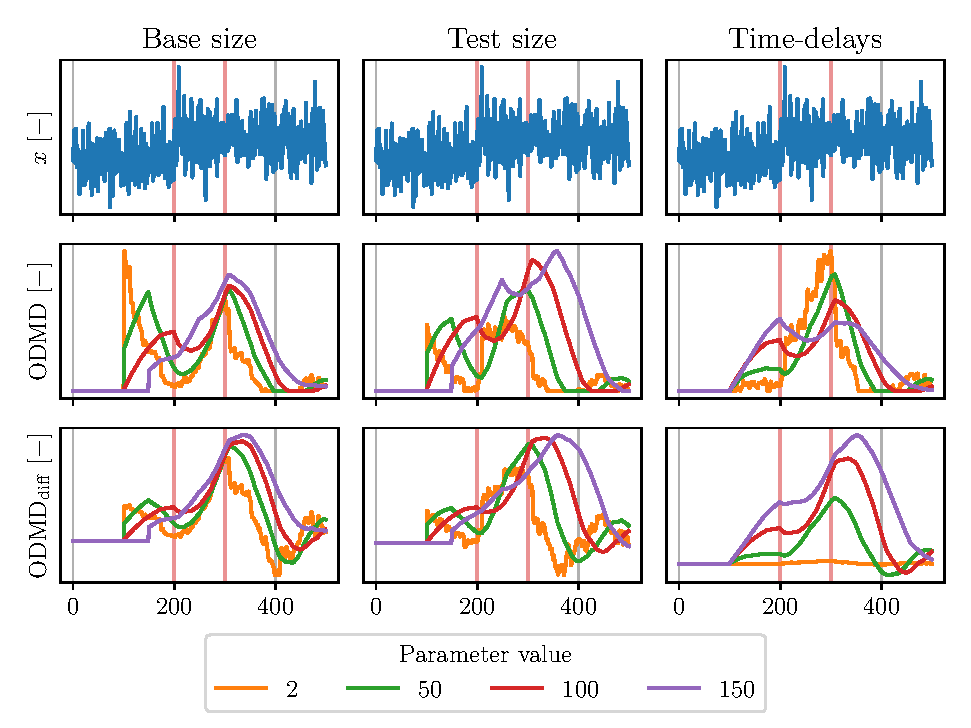
\includegraphics[width=\linewidth]{figures/Unit-step-parameters-influence-ref_size_test_size_hn.pdf}
	\caption{The influence of changing hyperparameter (denoted in the title of each column) values on CPD in synthetic unit step dataset.~Increasing value of base size stabilizes the score without significantly delaying the peak of CPD.~Increasing test size and number of time-delays in embedding increases robustness to noise more prominently while delaying the peak of CPD.}\label{fig:hyperparameters}
\end{figure}

\subsubsection{Approximating rank}
Determining the approximate rank \( r \) of the low-rank representation of the system is a crucial and inherently subjective step in any dimensionality reduction technique. To address this challenge, we recommend employing the systematic hard-thresholding algorithm proposed by Gavish and Donoho (2014) for extracting \( r \) from noisy data. This algorithm requires information about the ratio of the number of states \((m + l) h\) in the learning set \(\ui{\bar{X}}{L}\) and the learning window size \(a\), the selection of which is discussed later in Subsection~\ref{sec:base-window}.

Nevertheless, the proposed \( r \) may become computationally intractable for time-delayed embeddings. In such cases, we suggest using the row rank of the original data matrix \( m \) or, for augmented matrices, \( m + l \), in combination with hard-thresholding techniques to determine the optimal rank, particularly when linear system assumptions hold. For non-linear systems or situations where the collected data inadequately represent the underlying dynamics, a higher rank may be warranted to capture the dynamics effectively, while considering computational constraints and delayed response delivery. The online nature of the algorithm enables real-time adjustments to the rank, up to a certain threshold based on the significance of the \(r + 1\) singular value. These updates are facilitated by online singular value decomposition (SVD) algorithms, such as those presented in \cite{Brand2006} and \cite{Zhang2022}. For details on the implementation of rank-increasing updates, we refer readers to the original papers. Computational analysis by \cite{Zhang2019}, which applies for our proposed truncated version replacing number of states \(m\) with rank \(r\), indicates that the computational time of DMD updates scales with \( \mathcal{O}(r^2) \), with a number of floating-point multiplies of \(4n^2\), and memory requirements scale with \( \mathcal{O}(a r + 2 r ^ 2) \). This analysis can be utilized to evaluate the maximum rank for a given problem.

\subsubsection{Learning window size}
The learning window size \(d\) significantly influences the validity of the identified subspace and the accuracy of change-point detection. For identifying time-invariant systems, the learning window size should be sufficient to distinguish signal from noise and obtain the best approximation of the eigenvalues of the generating mechanism. For time-varying systems, the window size should encompass snapshots of single operating regimes or closely related operating regimes for effective learning. We propose setting the size of the base window as the lower bound on the learning window, although theoretically, the learning window could be smaller. The upper bound \(k >= b + c + d\) is determined by the number of available data points before the test window size \(c\) delayed by \(b\), as well as the size of the test window and the delay between the test and base windows. In summary, the learning window should be large enough to capture the system's dynamics without overlapping multiple operating states with distinct characteristics.

\subsubsection{Base window size and location}\label{sec:base-window}
The base window size \(a\) should reflect the expected duration of a stationary signal (single operation regime) within snapshots. This enables the reconstruction error of the base set to serve as a reference for the overall quality of the identified subspace and mitigates adverse effects on prediction accuracy. The base window should be located directly after the test window (\(b = 0\)). A value of \(a \leq d\) could prevent negative scores in collective anomalies, enabling effective differentiation between change points and collective changes.

\subsubsection{Test window size}
The test window size \(c\) determines the smoothness of change-point statistics over time. A larger test window results in smoother change-point statistics~\cite{Moskvina2003}. The selection of the test window size should consider the expected duration of the change-point, the nature of structural changes, and the desired smoothness of change-point statistics. Ideally, the peak of the statistics aligns precisely with the test window size delay from the change point. Smaller values of \(c\) decrease the delay, enhancing rapid detection but potentially missing slow drifts due to trends. Conversely, larger values of \(c\) increase stability and reduce false positives while potentially increasing false negative rates.

\subsubsection{Number of time-delays}
The number of time delays (\(h\)) is a critical parameter for ODMD-CPD in applications to non-linear systems with delayed effect of control action. Its selection relies on assumptions regarding the representativeness of snapshots with respect to the generating mechanism and the maximum expected delay of the control effect on system states. In the absence of such knowledge and with a reasonably large \(a\), \cite{Moskvina2003} recommend setting \(h = a / 2\) for the rank of the Hankel matrix. For larger \(a\), delay steps \(h_d\) may be used to capture the broadband dynamics of the system more effectively. The choice of \(h_d\) should be based on the maximum allowed number of features \((m + l)\frac{h}{h_d}\).

\subsubsection{Change-detection statistics threshold}
The threshold on change-detection statistics directly impacts the number of false positive or false negative alarms. Its proper selection further determines the delay of the detection alarm, as the rising change-point detection statistics cross the lower threshold sooner. As the CPD statistic, defined in Subsection~\ref{detect-cpd}, has no proper normalization and is influenced by the selection of other hyperparameters, the specification of constant values is challenging. As a general rule of thumb, higher recall (lower false negative rate) is achieved by setting the threshold lower. In contrast, higher precision (lower false positive rate) is achieved by setting the threshold higher. If accurate system tracking is achieved, i.e., \( r \) and \(h\) were selected so that the signal is extracted from noise well, the threshold could be set to zero while not compromising precision significantly. This may be desired in safety critical systems where higher recall helps to protect assets and life. Generally, the threshold should be set based on the desired trade-off between precision and recall, the change point's expected duration, and the structural changes' nature.
